% This file was created with tikzplotlib v0.9.17.
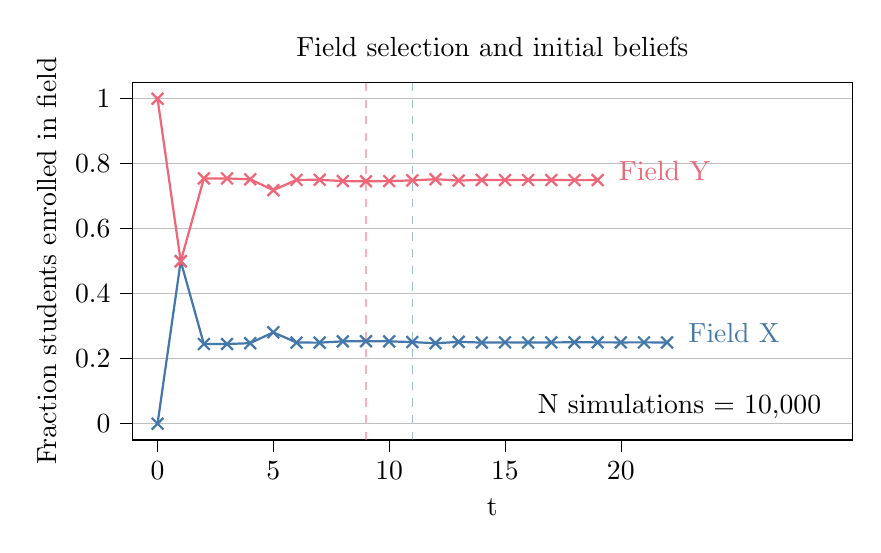
\begin{tikzpicture}

\definecolor{color0}{rgb}{0.266666666666667,0.466666666666667,0.666666666666667}
\definecolor{color1}{rgb}{0.933333333333333,0.4,0.466666666666667}

\begin{axis}[
height=6.121302808757603cm,
tick align=outside,
tick pos=left,
title={Field selection and initial beliefs},
unbounded coords=jump,
width=10.729849cm,
x grid style={white!69.0196078431373!black},
xlabel={t},
xmin=-1.1, xmax=30,
xtick style={color=black},
xtick={0,5,10,15,20},
xticklabels={
  \(\displaystyle 0\),
  \(\displaystyle 5\),
  \(\displaystyle 10\),
  \(\displaystyle 15\),
  \(\displaystyle 20\)
},
ylabel={Fraction students enrolled in field},
ymajorgrids,
ymin=-0.05, ymax=1.05,
ytick style={color=black},
ytick={0,0.2,0.4,0.6,0.8,1},
yticklabels={
  \(\displaystyle 0\),
  \(\displaystyle 0.2\),
  \(\displaystyle 0.4\),
  \(\displaystyle 0.6\),
  \(\displaystyle 0.8\),
  \(\displaystyle 1\)
}
]
\addplot [thick, color0, mark=x, mark size=3, mark options={solid}]
table {%
0 0
1 0.5003
2 0.2452
3 0.2452
4 0.2479
5 0.2813
6 0.2497
7 0.2495
8 0.2534
9 0.2539
10 0.2534
11 0.2512
12 0.2476
13 0.2518
14 0.2497
15 0.2503
16 0.25
17 0.2502
18 0.2505
19 0.2503
20 0.2502
21 0.2503
22 0.2501
};
\addplot [thick, color1, mark=x, mark size=3, mark options={solid}]
table {%
0 1
1 0.4997
2 0.7548
3 0.7548
4 0.7521
5 0.7187
6 0.7503
7 0.7505
8 0.7466
9 0.7461
10 0.7466
11 0.7488
12 0.7524
13 0.7482
14 0.7503
15 0.7497
16 0.75
17 0.7498
18 0.7495
19 0.7497
20 nan
21 nan
22 nan
};
\addplot [semithick, color0, opacity=0.5, dashed]
table {%
11 -0.05
11 1.05
};
\addplot [semithick, color1, opacity=0.5, dashed]
table {%
9 -0.05
9 1.05
};
\draw (axis cs:22.5,0.2501) node[
  anchor=base west,
  text=color0,
  rotate=0.0
]{Field X};
\draw (axis cs:19.5,0.7497) node[
  anchor=base west,
  text=color1,
  rotate=0.0
]{Field Y};
\draw (axis cs:16,0.03) node[
  anchor=base west,
  text=black,
  rotate=0.0
]{N simulations = 10,000};
\end{axis}

\end{tikzpicture}
